\documentclass[journal, a4paper]{IEEEtran}
\newcommand{\specialcell}[2][c]{%
  \begin{tabular}[#1]{@{}c@{}}#2\end{tabular}}
% some very useful LaTeX packages include:

%\usepackage{cite}      % Written by Donald Arseneau
                        % V1.6 and later of IEEEtran pre-defines the format
                        % of the cite.sty package \cite{} output to follow
                        % that of IEEE. Loading the cite package will
                        % result in citation numbers being automatically
                        % sorted and properly "ranged". i.e.,
                        % [1], [9], [2], [7], [5], [6]
                        % (without using cite.sty)
                        % will become:
                        % [1], [2], [5]--[7], [9] (using cite.sty)
                        % cite.sty's \cite will automatically add leading
                        % space, if needed. Use cite.sty's noadjust option
                        % (cite.sty V3.8 and later) if you want to turn this
                        % off. cite.sty is already installed on most LaTeX
                        % systems. The latest version can be obtained at:
                        % http://www.ctan.org/tex-archive/macros/latex/contrib/supported/cite/
                        
\usepackage{graphicx}
\usepackage{wrapfig}

\usepackage[T2A]{fontenc}			% кодировка
\usepackage[utf8]{inputenc}			% кодировка исходного текста
\usepackage[english,russian]{babel}	% локализация и переносы
\usepackage{graphicx}   % Written by David Carlisle and Sebastian Rahtz
                        % Required if you want graphics, photos, etc.
                        % graphicx.sty is already installed on most LaTeX
                        % systems. The latest version and documentation can
                        % be obtained at:
                        % http://www.ctan.org/tex-archive/macros/latex/required/graphics/
                        % Another good source of documentation is "Using
                        % Imported Graphics in LaTeX2e" by Keith Reckdahl
                        % which can be found as esplatex.ps and epslatex.pdf
                        % at: http://www.ctan.org/tex-archive/info/

%\usepackage{psfrag}    % Written by Craig Barratt, Michael C. Grant,
                        % and David Carlisle
                        % This package allows you to substitute LaTeX
                        % commands for text in imported EPS graphic files.
                        % In this way, LaTeX symbols can be placed into
                        % graphics that have been generated by other
                        % applications. You must use latex->dvips->ps2pdf
                        % workflow (not direct pdf output from pdflatex) if
                        % you wish to use this capability because it works
                        % via some PostScript tricks. Alternatively, the
                        % graphics could be processed as separate files via
                        % psfrag and dvips, then converted to PDF for
                        % inclusion in the main file which uses pdflatex.
                        % Docs are in "The PSfrag System" by Michael C. Grant
                        % and David Carlisle. There is also some information
                        % about using psfrag in "Using Imported Graphics in
                        % LaTeX2e" by Keith Reckdahl which documents the
                        % graphicx package (see above). The psfrag package
                        % and documentation can be obtained at:
                        % http://www.ctan.org/tex-archive/macros/latex/contrib/supported/psfrag/

%\usepackage{subfigure} % Written by Steven Douglas Cochran
                        % This package makes it easy to put subfigures
                        % in your figures. i.e., "figure 1a and 1b"
                        % Docs are in "Using Imported Graphics in LaTeX2e"
                        % by Keith Reckdahl which also documents the graphicx
                        % package (see above). subfigure.sty is already
                        % installed on most LaTeX systems. The latest version
                        % and documentation can be obtained at:
                        % http://www.ctan.org/tex-archive/macros/latex/contrib/supported/subfigure/

\usepackage{url}        % Written by Donald Arseneau
                        % Provides better support for handling and breaking
                        % URLs. url.sty is already installed on most LaTeX
                        % systems. The latest version can be obtained at:
                        % http://www.ctan.org/tex-archive/macros/latex/contrib/other/misc/
                        % Read the url.sty source comments for usage information.

%\usepackage{stfloats}  % Written by Sigitas Tolusis
                        % Gives LaTeX2e the ability to do double column
                        % floats at the bottom of the page as well as the top.
                        % (e.g., "\begin{figure*}[!b]" is not normally
                        % possible in LaTeX2e). This is an invasive package
                        % which rewrites many portions of the LaTeX2e output
                        % routines. It may not work with other packages that
                        % modify the LaTeX2e output routine and/or with other
                        % versions of LaTeX. The latest version and
                        % documentation can be obtained at:
                        % http://www.ctan.org/tex-archive/macros/latex/contrib/supported/sttools/
                        % Documentation is contained in the stfloats.sty
                        % comments as well as in the presfull.pdf file.
                        % Do not use the stfloats baselinefloat ability as
                        % IEEE does not allow \baselineskip to stretch.
                        % Authors submitting work to the IEEE should note
                        % that IEEE rarely uses double column equations and
                        % that authors should try to avoid such use.
                        % Do not be tempted to use the cuted.sty or
                        % midfloat.sty package (by the same author) as IEEE
                        % does not format its papers in such ways.

\usepackage{amsmath}    % From the American Mathematical Society
                        % A popular package that provides many helpful commands
                        % for dealing with mathematics. Note that the AMSmath
                        % package sets \interdisplaylinepenalty to 10000 thus
                        % preventing page breaks from occurring within multiline
                        % equations. Use:
%\interdisplaylinepenalty=2500
                        % after loading amsmath to restore such page breaks
                        % as IEEEtran.cls normally does. amsmath.sty is already
                        % installed on most LaTeX systems. The latest version
                        % and documentation can be obtained at:
                        % http://www.ctan.org/tex-archive/macros/latex/required/amslatex/math/



% Other popular packages for formatting tables and equations include:

%\usepackage{array}
% Frank Mittelbach's and David Carlisle's array.sty which improves the
% LaTeX2e array and tabular environments to provide better appearances and
% additional user controls. array.sty is already installed on most systems.
% The latest version and documentation can be obtained at:
% http://www.ctan.org/tex-archive/macros/latex/required/tools/

% V1.6 of IEEEtran contains the IEEEeqnarray family of commands that can
% be used to generate multiline equations as well as matrices, tables, etc.

% Also of notable interest:
% Scott Pakin's eqparbox package for creating (automatically sized) equal
% width boxes. Available:
% http://www.ctan.org/tex-archive/macros/latex/contrib/supported/eqparbox/

% *** Do not adjust lengths that control margins, column widths, etc. ***
% *** Do not use packages that alter fonts (such as pslatex).         ***
% There should be no need to do such things with IEEEtran.cls V1.6 and later.
\usepackage{soul}
\usepackage{soulutf8}

\usepackage{ amssymb }
% Your document starts here!
\begin{document}

% Define document title and author
	\title{{\large Лабораторная работа № 4.3.2}\\Дифракция света на ультразвуковой волне в
жидкости
}
	\author{Ступаков Олег \hspace{11cm} ~8 февраля 2019 г. \\ 722 группа 
	\hspace{11.71cm} ~г. Долгопрудный~
	\thanks{\fbox{Установка с вертикальной щелью}}}
	\markboth{{\small П}осле прочтения уничтожить {\small }}{}
	\maketitle

% Write abstract here
%\begin{abstract}

%\end{abstract}

% Each section begins with a \section{title} command
\section*{}
	% \PARstart{}{} creates a tall first letter for this first paragraph
	\PARstart{}{~Ц{\small ель работы}}{\large :} изучение дифракции света на синусоидальной акустической решетке и наблюдение фазовой решетки методом темного поля.\vspace{0.15cm}
	\PARstart{}{{\footnotesize ~}O{\small борудование}}{\large :}~оптическая скамья, осветитель, два длиннофокусных объектива, кювета с
жидкостью, кварцевый излучатель с микрометрическим винтом, генератор звуковой частоты,
линза, вертикальная нить на рейтере, микроскоп.
% Main Part
\section{Теоретическое введение}
	При прохождении ультразвуковой волны через жидкость в ней возникают периодические неоднородности коэффициента преломления, создается фазовая решетка, которую мы считаем неподвижной ввиду малости скорости звука относительно скорости света. Показатель
	преломления n изменяется по закону:
	
	\begin{equation}\label{}
	n = n_0 (1 + m \cos \Omega x)
	\end{equation}
	
	Здесь $ \Omega = 2 \pi / \Lambda $ --- волновое число для ультразвуковой волны, $ m $ --- глубина модуляции $ n $ $ (m \ll 1 $).
	
	Положим фазу $ \phi $ колебаний световой волны на передней стенке кюветы равной нулю, тогда на задней поверхности она равна:
	
	\begin{equation}\label{}
	\phi  = k n L = \phi_0 (1 + m \cos \Omega x)
	\end{equation}
	
	Здесь $ L $ --- толщина жидкости в кювете, $ k = 2 \pi / \lambda $ --- волновое число для света.
	
	После прохождения через кювету световое поле есть совокупность плоских волн, распространяющихся под углами $ \theta $, соответствующими максимумам в дифракции Фраунгофера:
	
\begin{equation}\label{}	
	\Lambda \sin \theta_m = m \lambda
\end{equation}

	Этот эффект проиллюстрирован на рисунке 1.
	\begin{figure}[h!]
		\centering	
		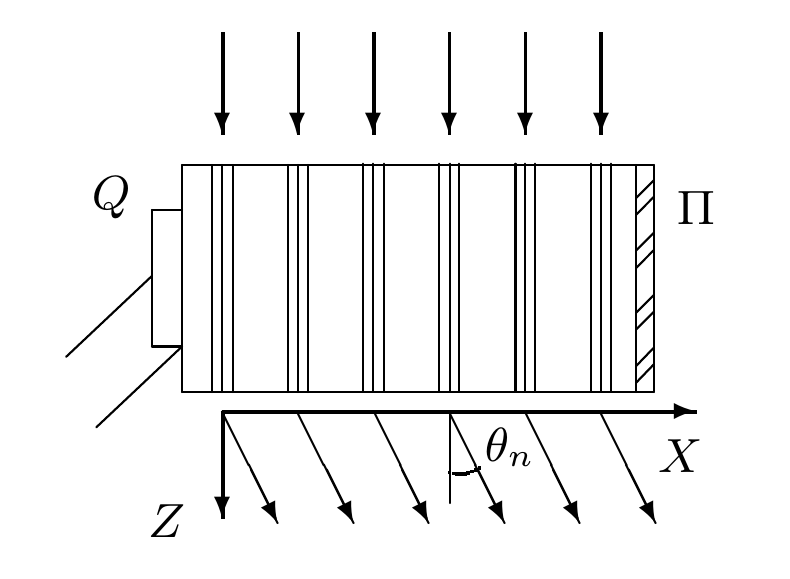
\includegraphics[width=0.3\textwidth]{difraction.png}
		\caption{Дифракция световых волн на акустической решетке}
		\label{diff}
	\end{figure}

	Зная положение дифракционных максимумов, по формуле (1) легко определить длину ультразвуковой волны, учитывая малость $ \theta $: $ \sin \theta \approx \theta \approx l_m /F  $, где $ l_m $ --- расстояние от нулевого до последнего видимого максимума, $ F $ --- фокусное расстояние линзы. Тогда получим:
	
	\begin{equation}\label{}
	 \Lambda = m \lambda F/ l_m 
	\end{equation}
	Скорость ультразвуковых волн в жидкости, где $ \nu $ --- частота колебаний излучателя:
	
\begin{equation}\label{}
	v = \Lambda \nu 
\end{equation}

\section{Определение скорости ультразвука по дифракционной картине}
	
Схема установки приведена на рисунке 2. Источник света Л через светофильтр Ф и конденсор К освещает вертикальную щель $ S $, находящуюся в фокусе объектива $ O_1 $. После объектива параллельный световой пучок проходит через кювету С перпендикулярно акустической решетке, и дифракционная картина собирается в фокальной плоскости объектива $ O_2 $ , наблюдается при помощи микроскопа М.

Предварительную настройку установки произведем в соответствии с инструкцией с зеленым фильтром, далее в работе используется красный.

	\begin{figure}[h!]
	\centering	
	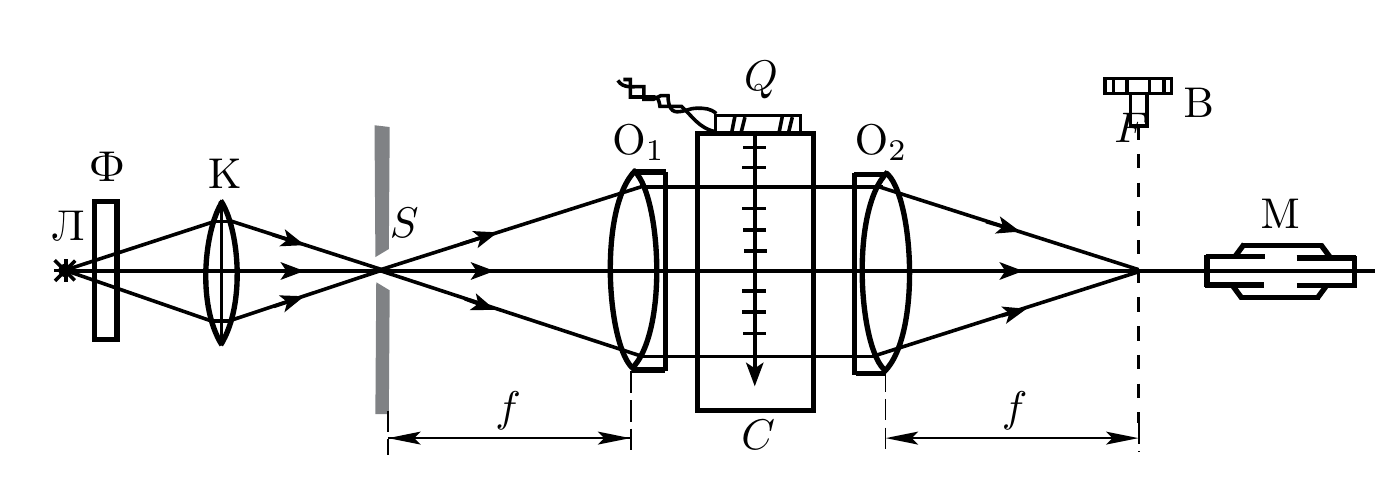
\includegraphics[width=0.53\textwidth]{shema1.png}
	\caption{Схема для наблюдения дифракции на акустической решетке}
	\label{shema1}
\end{figure}

Параметры установки: фокусное расстояние объектива $  O_2  $ $ F = 30 $ см, одно деление винта микроскопа составляет 4 мкм, погрешность измерений примем равной  $ \sigma = $ 2 деления, или 8 мкм.

Исследуем изменения дифракционной картины на зеленом свете. При увеличении частоты УЗ-генератора и приближении к 1,1 МГц проявляется дифракционная решетка: расстояние между максимумами растет.

Измерим положения $ x_m $ дифракционных максимумов с помощью микроскопического винта для четырех частот. Результаты измерений занесены в таблицы {\footnotesize I-IV} ниже. На основе каждой таблицы построены графики зависимости $ x_m (m) $, они изображены на рисунках 3-6. Коэффициенты углов наклонов прямых для всех зависимостей сведены в таблицу {\small V}. 

	\begin{table}[h!]
	\centering
	\begin{tabular}{|c|c|c|c|c|c|c|c|}
\hline
$m$&-3&-2&-1&0&1&2&3\\
\hline
$x_m$, дел&-115&-78&-37&0&38&74&106\\
\hline
$x_m$, мкм&-460&-312&-148&0&152&296&424\\
\hline
\end{tabular}

	\caption{Измерение координаты $ m $-ого максимума $ x_m $ дифракционной картины при частоте генератора $ \nu = $ 1,168 МГц}
	\label{nu1}
\end{table}	

	\begin{figure}[h!]
	\centering
	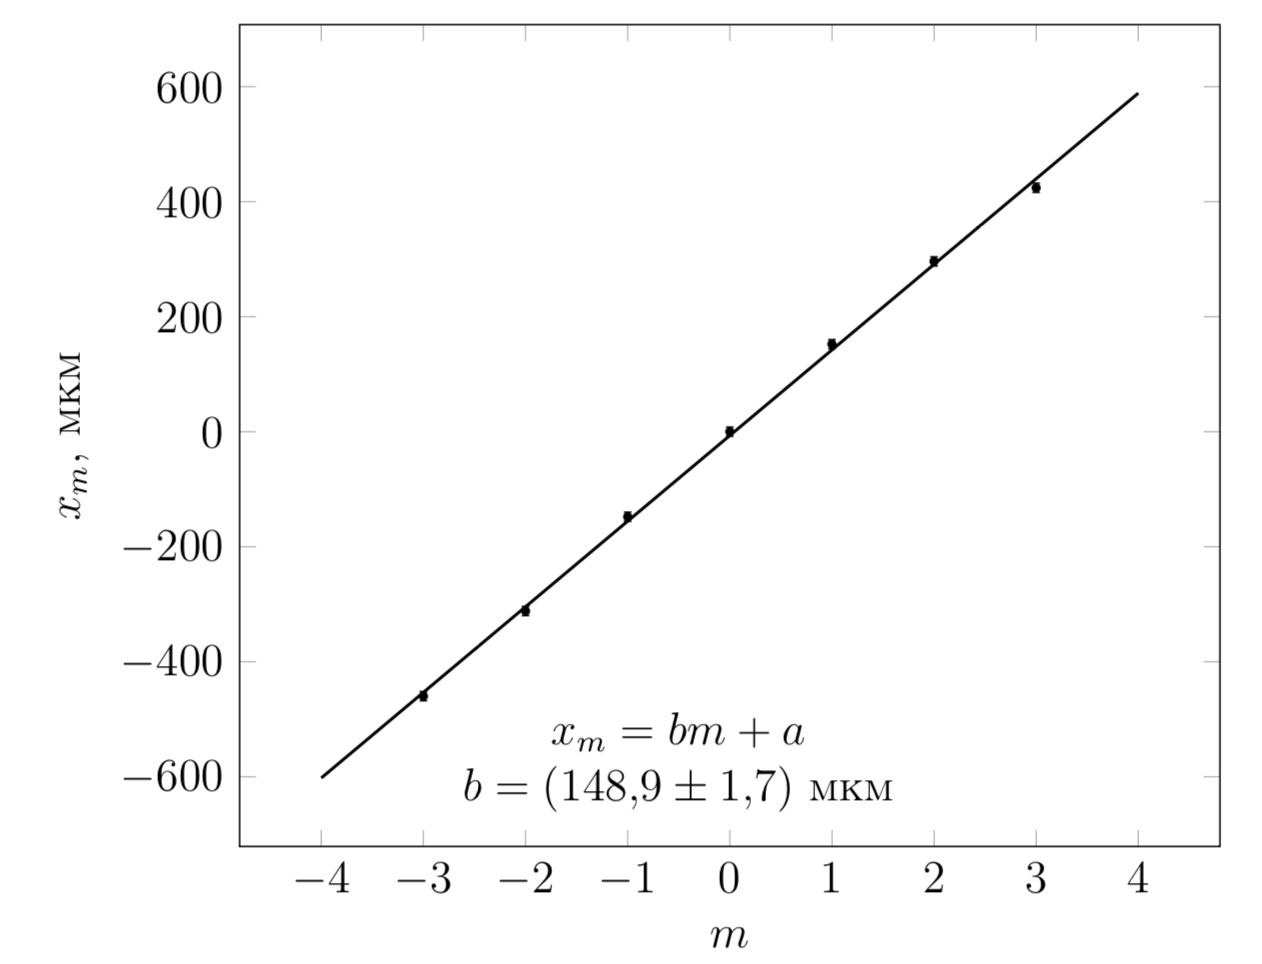
\includegraphics[width=1.02\linewidth]{1.png}
	\caption{График зависимости $  x_m(m) $ при частоте генератора $ \nu = $ 1,168 МГц}
	\label{nu1_graf}
\end{figure}
	
		\begin{table}[h!]
		\centering
		\begin{tabular}{|p{12pt}|c|c|c|c|c|c|c|c|c|}
\hline
$m$&-4&-3&-2&-1&0&1&2&3&4\\
\hline
$x_m$, дел&-150&-116&-81&-38&0&38&80&120&154\\
\hline
$x_m$, мкм&-600&-464&-324&-152&0&152&320&480&616\\
\hline
\end{tabular}

		\caption{Измерение координаты $ m $-ого максимума $ x_m $ дифракционной картины при частоте генератора $ \nu = $ 1,219 МГц}
		\label{nu2}
	\end{table}	
	Ошибка при определении $ \Lambda $ и $ v $ не превышает 2\%. Согласно справочным данным, при комнатной температуре скорость ультразвуковой волны в воде составляет примерно 1490 м/с. Значения, полученные экспериментально, с достаточной точностью соотносятся с ними.

\begin{figure}[h!]
	\centering
	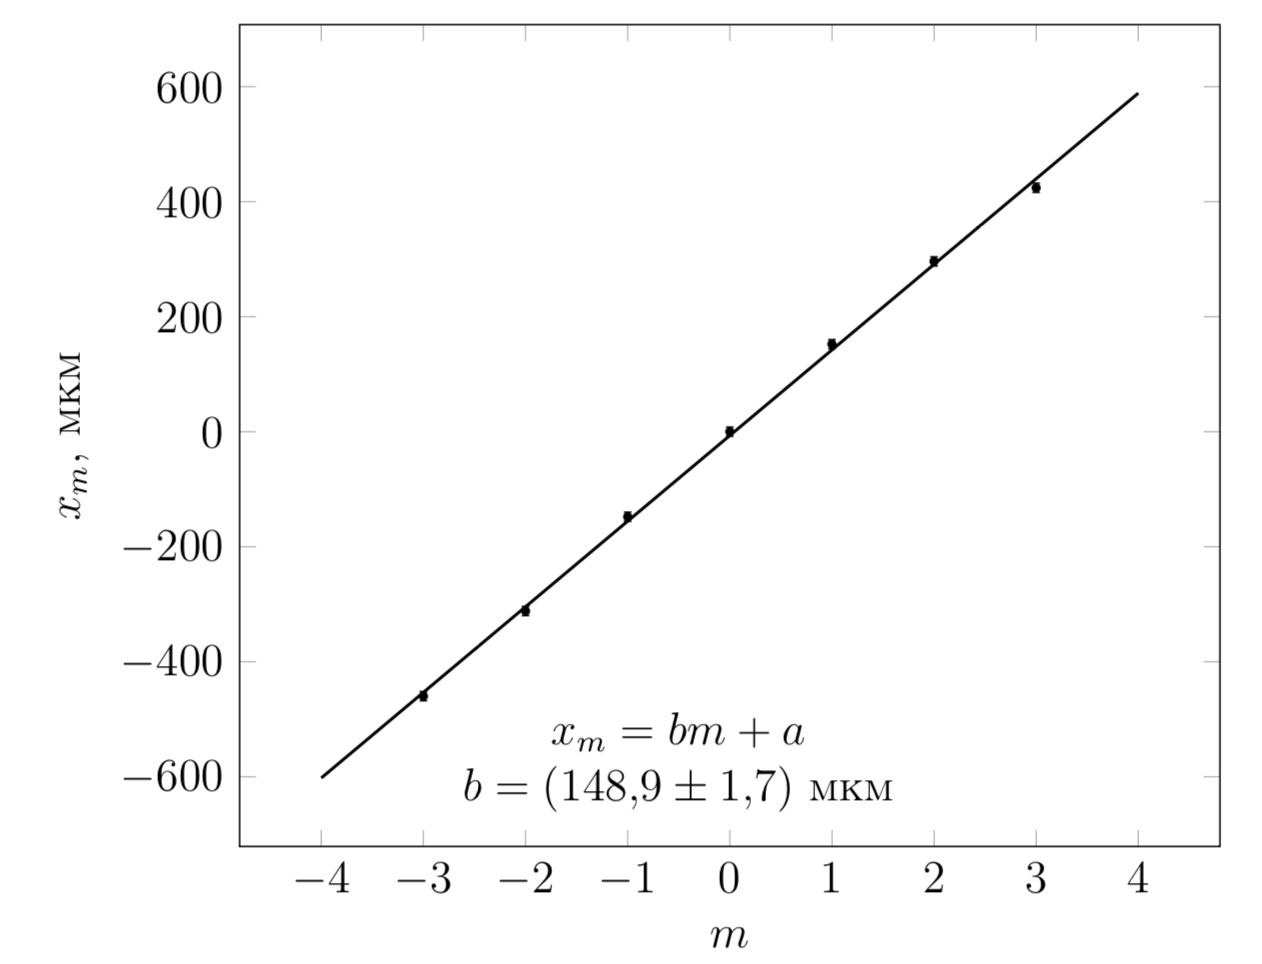
\includegraphics[width=1.02\linewidth]{1.png}
	\caption{График зависимости $  x_m(m) $ при частоте генератора $ \nu = $ 1,219 МГц}
	\label{nu2_graf}
\end{figure}

		\begin{table}[h!]
		\centering
		\begin{tabular}{|c|c|c|c|c|c|c|c|}
\hline
$m$&-3&-2&-1&0&1&2&3\\
\hline
$x_m$, дел&-116&-80&-38&0&45&86&126\\
\hline
$x_m$, мкм&-464&-320&-152&0&180&344&504\\
\hline
\end{tabular}
		\caption{Измерение координаты $ m $-ого максимума $ x_m $ дифракционной картины при частоте генератора $ \nu = $ 1,248 МГц}
		\label{nu3}
	\end{table}	

\begin{figure}[h!]
	\centering
	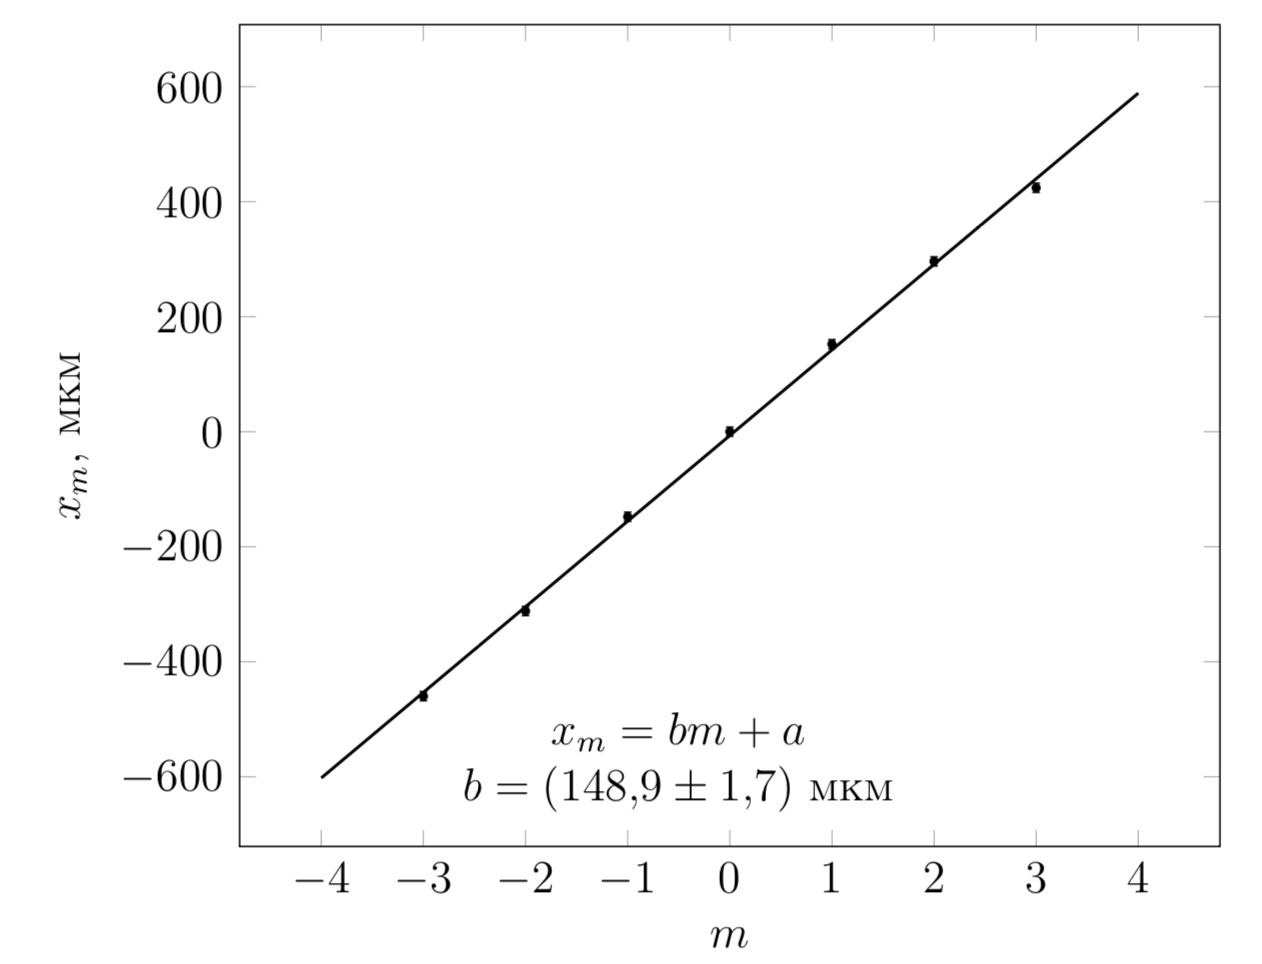
\includegraphics[width=1.02\linewidth]{1.png}
	\caption{График зависимость$  x_m(m) $ при частоте генератора $ \nu = $ 1,248 МГц}
	\label{nu3_graf}
\end{figure}
\


	\begin{table}[h!]
	\centering
	\begin{tabular}{|c|c|c|c|c|c|}
\hline
$m$&-2&-1&0&1&2\\
\hline
$x_m$, дел&-94&-43&0&45&85\\
\hline
$x_m$, мкм&-376&-172&0&180&340\\
\hline
\end{tabular}
	\caption{~~~~Измерение координаты $ m $-ого максимума $ x_m $ дифракционной картины при частоте генератора $ \nu = $ 1,331 МГц}
	\label{nu4}
\end{table}	

\begin{figure}[h!]
	\centering
	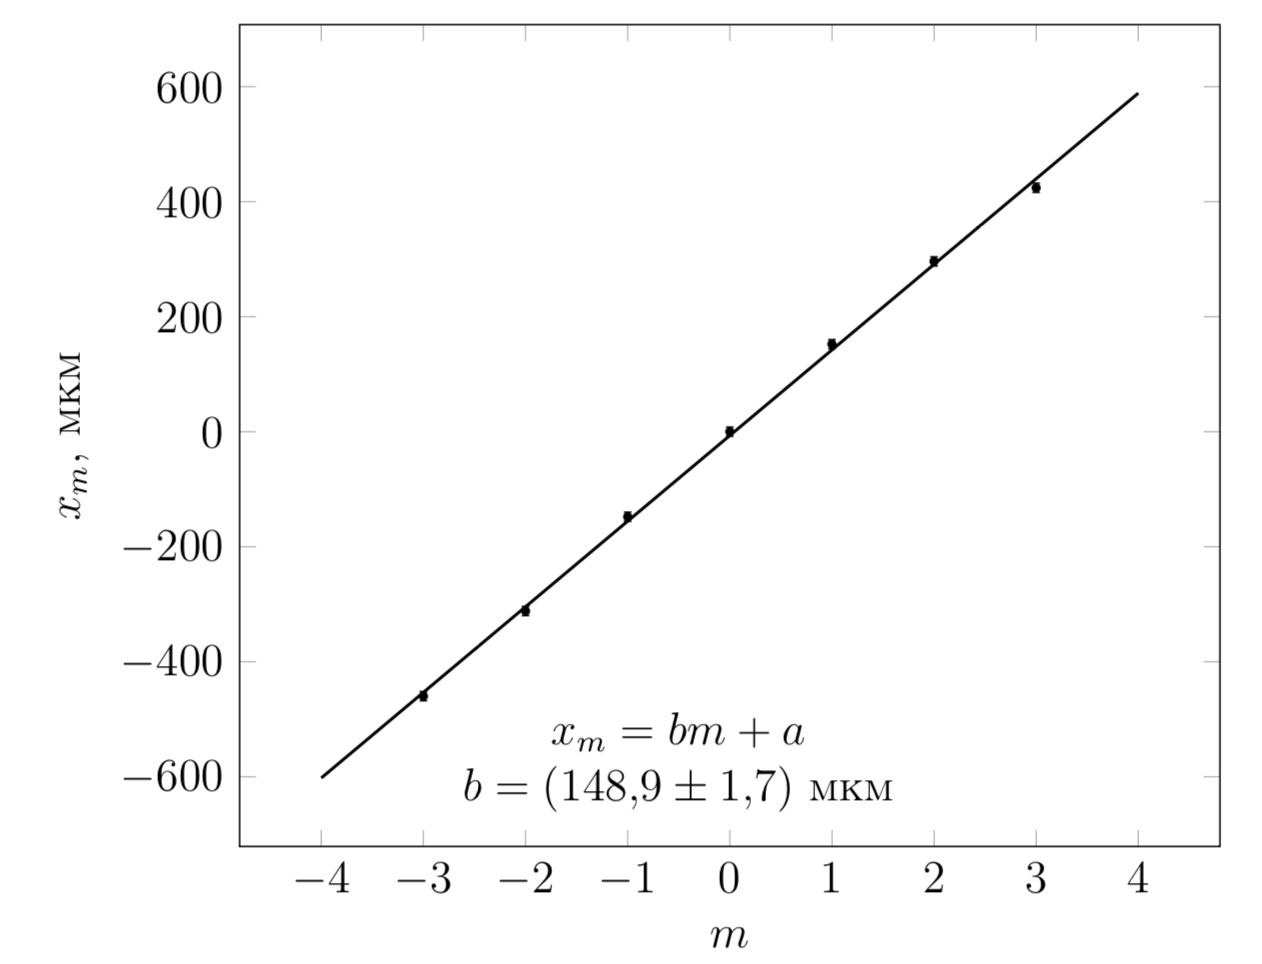
\includegraphics[width=1.02\linewidth]{1.png}
	\caption{График зависимость$  x_m(m) $ при частоте генератора $ \nu = $ 1,331 МГц}
	\label{nu4_graf}
\end{figure}

	\begin{table}[h!]
	\centering
	\begin{tabular}{|c|c|c|c|c|c|c|c|c|c|c|}
\hline
$\nu$, МГц&$b$, мкм&$\sigma_b$, мкм&$\Lambda$, мкм&$\Delta \Lambda$, мкм&$v$, м/с&$\Delta v$, м/с\\
\hline
1,168&148,9&1,6&1289&15&1507&15\\
\hline
1,219&154,8&1,3&1240&10&1512&13\\
\hline
1,258&163,0&1,4&1178&10&1482&13\\
\hline
1,331&178&3&1076&20&1432&30\\
\hline
\end{tabular}
	\caption{Вычисление длины ультразвуковой волны $ \Lambda $ и скорости распространения ее в воде $ v $}
	\label{speed}
\end{table}	


\section{Определение скорости ультразвука методом темного поля}
	
Для наблюдения акустической решетки используется метод темного поля, который заключается в устранении центрального дифракционного максимума с помощью непрозрачного экрана. Схема установки показана на рисунке 7.

	\begin{figure}[h!]
	\centering	
	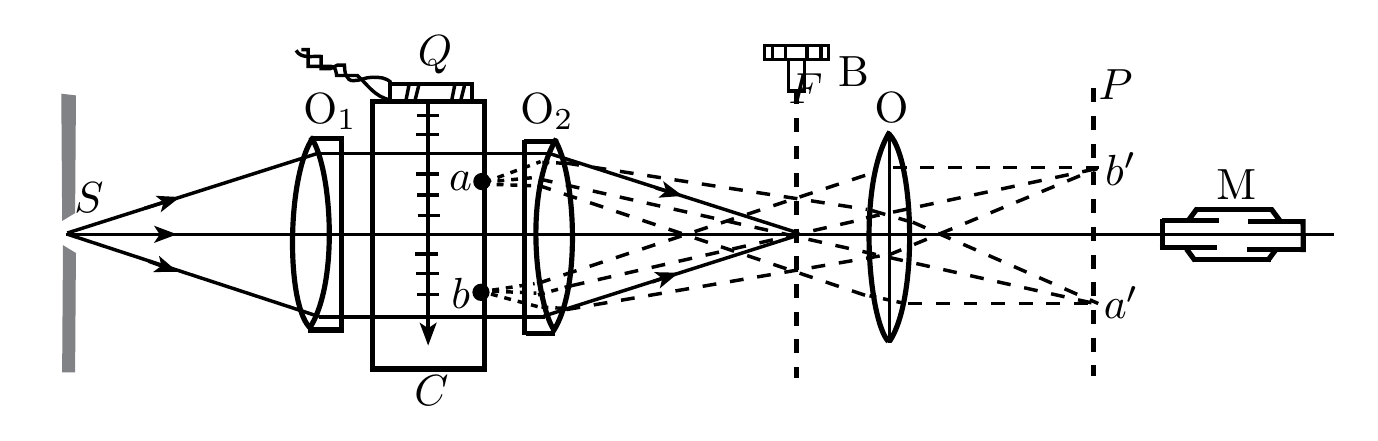
\includegraphics[width=0.5\textwidth]{shema2.png}
	\caption{Схема для наблюдения дифракции методом темного поля}
	\label{shema2}
\end{figure}

Приставим к задней стенке (для светового луча) кюветы стеклянную пластинку с миллиметровыми делениями; сфокусируем микроскоп на изображение пластинки. Определим цену деления окулярной шкалы микроскопа, совместив ее с миллиметровыми делениями: в 6 делениях миллиметровой шкалы убирается 100 маленьких делений окулярной. Значит, цена деления окулярной шкалы: $ C = $ 0,06 мм.

Без применения метода темного поля звуковая решетка не наблюдается. Закроем нулевой максимум горизонтальной нитью. Таким образом, осевая составляющая фазово-модулированной волны поглощается, а боковые остаются без изменения. Получившееся поле: 

\begin{equation}\label{}
\begin{aligned}
f(x) = \dfrac{im}{2} e^{i\Omega x} +  &\dfrac{im}{2} e^{-i\Omega x} = im\\ \Downarrow&\\
I(x) = m^2 \cos ^2 \Omega x = &m^2 \dfrac{1 + \cos ^2 2 \Omega x}{2}
\end{aligned}
\end{equation}

Отсюда получаем, что расстояние между темными полосами есть $ \Lambda/2 $.

Проведем измерение длины ультразвуковой волны, приняв ошибку равной цене деления окулярной шкалы. В таблице 6 содержатся количество маленьких делений окулярной шкалы N (цена деления $ C = 0,06 $), соответствующее $ n $ темным полосам акустической решетки.
Формулы для расчета длины волны ультразвука $ \Lambda $ и` скорости распространения $ v $ в воде:
\begin{equation}\label{}
\Lambda/2  = NC/(n - 1),  \qquad v = \nu\Lambda
\end{equation}

\,\,\,\,\,\,\,\,Расчеты также приведены в таблице VI. Ошибка\\ \hspace*{17pt} при таком определении скорости звука больше, \\ \hspace*{21pt}чем в первой части работы, и
составляет около 

\hspace*{12pt}5\%. Сами значения тоже получились больше.\\[0.3cm]

\begin{table}[h!]
	\centering
\begin{tabular}{|p{0.7cm}|p{2cm}|p{2cm}|p{0.7cm}|p{0.83cm}|p{0.83cm}|c|c|c|c|}
\hline
 \vspace{0.22cm} \hspace{5pt}$\nu$\hspace{2pt}, Мгц& Количество делений шкалы окуляра $N$&Количество темных полос акустической решетки $n$&\vspace{0.25cm} \hspace{2pt}$\Lambda$,мм&\vspace{0.25cm} \hspace{10pt}$v$, $10$~м/с&\vspace{0.21cm} \hspace{5pt}$\Delta v$, $10$~м/с\\
\hline
1,220&~~~~~150&~~~~~15&1,29&~157&~~6\\
\hline
1,259&~~~~~150&~~~~~16&1,20&~151&~~7\\
\hline
1,271&~~~~~175&~~~~~18&1,24&~157&~~7\\
\hline
\end{tabular}
	\caption{Вычисление длины ультразвуковой волны $ \Lambda $ и скорости распространения ее в воде $ v $ методом темного поля}
	\label{dark}
\end{table}
\section{Вывод}

В данной работе определялась скорость ультразвука в воде разными методами: с помощью дифракционной картины \fbox{ ($v_{\text{сред}}= 1480 \pm 20 $)м/с} и методом темного поля \fbox{($ v_{\text{сред}}^{\centerdot}=1550 \pm 70$)м/с.} Скорости, экспериментально определенные обоими методами,
совпадают с табличными значениями в пределах погрешности.



% Your document ends here!
\end{document}
